\documentclass[conference]{IEEEtran}

% Some very useful LaTeX packages include:
% (uncomment the ones you want to load)


\usepackage{cite}
\usepackage{adjustbox}
\usepackage{float}
\usepackage{booktabs}

% *** GRAPHICS RELATED PACKAGES ***
%
\ifCLASSINFOpdf
  % \usepackage[pdftex]{graphicx}
  % declare the path(s) where your graphic files are
  % \graphicspath{{../pdf/}{../jpeg/}}
  % and their extensions so you won't have to specify these with
  % every instance of \includegraphics
  % \DeclareGraphicsExtensions{.pdf,.jpeg,.png}
\else
  % or other class option (dvipsone, dvipdf, if not using dvips). graphicx
  % will default to the driver specified in the system graphics.cfg if no
  % driver is specified.
  % \usepackage[dvips]{graphicx}
  % declare the path(s) where your graphic files are
  % \graphicspath{{../eps/}}
  % and their extensions so you won't have to specify these with
  % every instance of \includegraphics
  % \DeclareGraphicsExtensions{.eps}
\fi
% graphicx was written by David Carlisle and Sebastian Rahtz. It is
% required if you want graphics, photos, etc. graphicx.sty is already
% installed on most LaTeX systems. The latest version and documentation
% can be obtained at: 
% http://www.ctan.org/pkg/graphicx
% Another good source of documentation is "Using Imported Graphics in
% LaTeX2e" by Keith Reckdahl which can be found at:
% http://www.ctan.org/pkg/epslatex
%
% latex, and pdflatex in dvi mode, support graphics in encapsulated
% postscript (.eps) format. pdflatex in pdf mode supports graphics
% in .pdf, .jpeg, .png and .mps (metapost) formats. Users should ensure
% that all non-photo figures use a vector format (.eps, .pdf, .mps) and
% not a bitmapped formats (.jpeg, .png). The IEEE frowns on bitmapped formats
% which can result in "jaggedy"/blurry rendering of lines and letters as
% well as large increases in file sizes.
%
% You can find documentation about the pdfTeX application at:
% http://www.tug.org/applications/pdftex





\usepackage{amsmath}

% *** SPECIALIZED LIST PACKAGES ***
%
%\usepackage{algorithmic}
% algorithmic.sty was written by Peter Williams and Rogerio Brito.
% This package provides an algorithmic environment fo describing algorithms.
% You can use the algorithmic environment in-text or within a figure
% environment to provide for a floating algorithm. Do NOT use the algorithm
% floating environment provided by algorithm.sty (by the same authors) or
% algorithm2e.sty (by Christophe Fiorio) as the IEEE does not use dedicated
% algorithm float types and packages that provide these will not provide
% correct IEEE style captions. The latest version and documentation of
% algorithmic.sty can be obtained at:
% http://www.ctan.org/pkg/algorithms
% Also of interest may be the (relatively newer and more customizable)
% algorithmicx.sty package by Szasz Janos:
% http://www.ctan.org/pkg/algorithmicx




% *** ALIGNMENT PACKAGES ***
%
%\usepackage{array}
% Frank Mittelbach's and David Carlisle's array.sty patches and improves
% the standard LaTeX2e array and tabular environments to provide better
% appearance and additional user controls. As the default LaTeX2e table
% generation code is lacking to the point of almost being broken with
% respect to the quality of the end results, all users are strongly
% advised to use an enhanced (at the very least that provided by array.sty)
% set of table tools. array.sty is already installed on most systems. The
% latest version and documentation can be obtained at:
% http://www.ctan.org/pkg/array


% IEEEtran contains the IEEEeqnarray family of commands that can be used to
% generate multiline equations as well as matrices, tables, etc., of high
% quality.




% *** SUBFIGURE PACKAGES ***
%\ifCLASSOPTIONcompsoc
%  \usepackage[caption=false,font=normalsize,labelfont=sf,textfont=sf]{subfig}
%\else
%  \usepackage[caption=false,font=footnotesize]{subfig}
%\fi
% subfig.sty, written by Steven Douglas Cochran, is the modern replacement
% for subfigure.sty, the latter of which is no longer maintained and is
% incompatible with some LaTeX packages including fixltx2e. However,
% subfig.sty requires and automatically loads Axel Sommerfeldt's caption.sty
% which will override IEEEtran.cls' handling of captions and this will result
% in non-IEEE style figure/table captions. To prevent this problem, be sure
% and invoke subfig.sty's "caption=false" package option (available since
% subfig.sty version 1.3, 2005/06/28) as this is will preserve IEEEtran.cls
% handling of captions.
% Note that the Computer Society format requires a larger sans serif font
% than the serif footnote size font used in traditional IEEE formatting
% and thus the need to invoke different subfig.sty package options depending
% on whether compsoc mode has been enabled.
%
% The latest version and documentation of subfig.sty can be obtained at:
% http://www.ctan.org/pkg/subfig




% *** FLOAT PACKAGES ***
%
%\usepackage{fixltx2e}
% fixltx2e, the successor to the earlier fix2col.sty, was written by
% Frank Mittelbach and David Carlisle. This package corrects a few problems
% in the LaTeX2e kernel, the most notable of which is that in current
% LaTeX2e releases, the ordering of single and double column floats is not
% guaranteed to be preserved. Thus, an unpatched LaTeX2e can allow a
% single column figure to be placed prior to an earlier double column
% figure.
% Be aware that LaTeX2e kernels dated 2015 and later have fixltx2e.sty's
% corrections already built into the system in which case a warning will
% be issued if an attempt is made to load fixltx2e.sty as it is no longer
% needed.
% The latest version and documentation can be found at:
% http://www.ctan.org/pkg/fixltx2e


%\usepackage{stfloats}
% stfloats.sty was written by Sigitas Tolusis. This package gives LaTeX2e
% the ability to do double column floats at the bottom of the page as well
% as the top. (e.g., "\begin{figure*}[!b]" is not normally possible in
% LaTeX2e). It also provides a command:
%\fnbelowfloat
% to enable the placement of footnotes below bottom floats (the standard
% LaTeX2e kernel puts them above bottom floats). This is an invasive package
% which rewrites many portions of the LaTeX2e float routines. It may not work
% with other packages that modify the LaTeX2e float routines. The latest
% version and documentation can be obtained at:
% http://www.ctan.org/pkg/stfloats
% Do not use the stfloats baselinefloat ability as the IEEE does not allow
% \baselineskip to stretch. Authors submitting work to the IEEE should note
% that the IEEE rarely uses double column equations and that authors should try
% to avoid such use. Do not be tempted to use the cuted.sty or midfloat.sty
% packages (also by Sigitas Tolusis) as the IEEE does not format its papers in
% such ways.
% Do not attempt to use stfloats with fixltx2e as they are incompatible.
% Instead, use Morten Hogholm'a dblfloatfix which combines the features
% of both fixltx2e and stfloats:
%
% \usepackage{dblfloatfix}
% The latest version can be found at:
% http://www.ctan.org/pkg/dblfloatfix

% *** PDF, URL AND HYPERLINK PACKAGES ***
%
\usepackage{url}
% Basically, \url{my_url_here}.


% for comments
\usepackage{color}
\newcommand{\mycomment}[3]{\emph{\textcolor{#2}{#1}: }\textcolor{#2}{#3}}
\newcommand{\todo}[1]{\mycomment{Todo}{red}{#1}}
\newcommand{\sangeetha}[1]{\mycomment{Sangeetha}{magenta}{#1}}
\newcommand{\eric}[1]{\mycomment{Eric}{cyan}{#1}}

% correct bad hyphenation here
\hyphenation{op-tical net-works semi-conduc-tor}


\begin{document}
% paper title
\title{On the Possibility of NLOS Reconstruction Using Spatial Decomposition\\ \Large{ECE901 Project}}


% author names and affiliations
% use a multiple column layout for up to three different
% affiliations
\author{
\IEEEauthorblockN{Eric Brandt}
\IEEEauthorblockA{University of Wisconsin, Madison\\
Email: \texttt{elbrandt@wisc.edu}}}


% make the title area
\maketitle



\begin{abstract}
Hidden scene reconstruction by non-line of sight imaging is a popular and growing field of computational optics. Capabilities for fast capture of large hidden scenes are improving, placing increasing pressure on efficient computational methods to reconstruct those scenes. Using current techniques, this reconstruction process is quite computationally expensive if performed in the time domain, having a $O(N^5)$ complexity in the straightforward implementation. This is a significant impediment to considering reconstruction of hidden scenes larger than a small room. We investigate the opportunities for reducing this computational cost by combining techniques of variable resolution reconstruction and spatial decomposition. Using existing data sets, we show that by using efficient data structures, an empirical computational lower bound on time domain reconstruction can be as low as 0.5\% of the cost of the straightforward implementation.
\end{abstract}

\section{Background}
Hidden scene reconstruction by use of non-line of sight imaging techniques is a popular sub-genre of computational optics research. A typical experimental setup involves a laser capable of emitting short pulses and a camera capable of measuring arrival times of single photons with very high accuracy. A very short pulse of laser light is directed to a relay surface, typically a wall. This coherent light is scattered in all directions when reflected off the relay surface into a scene that is not directly visible to the camera. Some of the scattered laser light bounces off of objects in the scene, some of which bounces back to the relay wall, and finally some of which is detected by the camera, as depicted in figure \ref{fig:2dsetup}. The difference between the emitted number of photons and the detected number of photons can be on the order of $10^{-15}$. Sequentially, the laser is aimed at many positions on the relay surface, usually in a grid-like pattern, at each of which a pulse is emitted and the camera detects and time-stamps the photons that have completed the three-bounce voyage from wall, to hidden scene, to relay wall, to camera. From this, a `3D-Impulse Response' cube of data can be collected. The first two dimensions of this response cube are the X- and Y- location of the originating pulse on the laser wall. The third dimension is the arrival time of each photon captured by the camera from the pulse at the particular X,Y location.

\begin{figure}
    \centering
    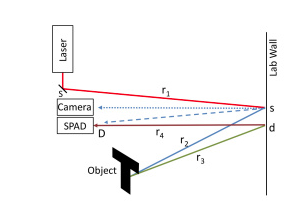
\includegraphics[width=\columnwidth]{figures/2dsetup.png}
    \caption{Diagram of photon path in typical NLOS experimental setup}
    \label{fig:2dsetup}
\end{figure}

Once the data is collected, any of several computational methods \cite{velten2012, Liu2019, Nam2020} can be used to reconstruct the hidden scene from the 3D-Impulse Response cube. Perhaps the most straightforward method is to perform backprojection in the time domain, described now: Consider a single relay wall location, and the 1D time-series of photon arrival times collected by the camera from the laser pulse directed at that relay wall location. We can mathematically construct a `virtual phasor pulse' as shown in figure \ref{fig:virtualpulse} and convolve this pulse with the 1D time series. This has the effect of simulating the sending of this virtual pulse through the scene. This convolution can be applied to the time-series collected for all X- and Y-locations on the relay wall, forming a data set representing how a laser pulse would travel through the scene. This is commonly known as the Virtual Phasor Field in literature \cite{Liu2019}.

\begin{figure}
    \centering
    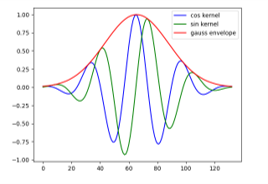
\includegraphics[width=0.6\columnwidth]{figures/phasor_pulse_short.png}
    \caption{Phasor pulse to be convolved with time impulse response}
    \label{fig:virtualpulse}
\end{figure}

Having this Virtual Phasor Field, we can reconstruct the hidden scene as follows: The hidden scene is spatially divided into voxels of a uniform dimension that is a function of the wavelength used in the virtual phasor pulse (see Proposed Method section for details). The reconstruction algorithm considers each voxel, which has a known 3D coordinate in the scene, and calculates the flux of photons that were captured by the camera as a result of reflection off of surfaces in that voxel. To do this, for a given voxel, the algorithm considers each relay wall location of laser pulses, and computes the distances $r_1$, $r_2$, $r_3$ , $r_4$ in figure \ref{fig:2dsetup}, where the distances $r_2$ and $r_3$ are determined by the location of the voxel and the laser position currently under consideration. The time-of-flight is calculated from the sum of these distances. The virtual Phasor Field is used as a sort of `lookup table' to find out if any, and how many, photons were recorded that would have an arrival time coinciding with being reflected by this voxel. Summing this lookup over all laser positions for a given voxel gives the intensity of reflection for that voxel. Repeating this for all voxels produces a 3D spatial cube of signal response which represents the reconstructed scene. For a 2D view of the reconstructed scene, the maximum intensity for each X,Y coordinate is selected along the corresponding Z depth. The resulting 2D image is then normalized and color-mapped for presentation. A typical reconstruction can be seen in figure \ref{fig:typscene} (source: \cite{Liu2019}).

\begin{figure}
    \centering
    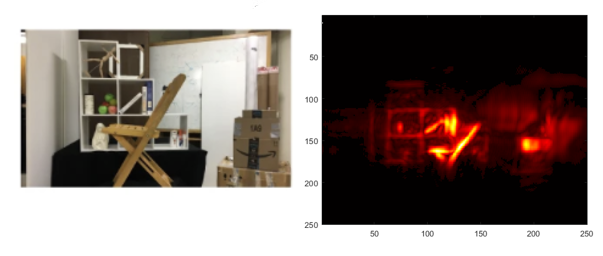
\includegraphics[width=\columnwidth]{figures/typscene.png}
    \caption{Left: Actual scene.  Right: NLOS Reconstruction}
    \label{fig:typscene}
\end{figure}

As can be seen in the algorithmic description above, the computation time required to perform the reconstruction is a product of the relay wall dimensions (e.g. $U \times V$) and the voxel scene dimensions (e.g. $X \times Y \times Z$), resulting in a computational complexity of $O(UVXYZ)$ or more compactly $O(N^5)$.

\section{Related Work}
Early work on non-line of sight imaging was pioneered by \cite{velten2012} who began the work of guiding an ultra-fast pulsed laser to multiple relay wall locations using a galvo. In their work, a streak camera was used as the detector. This work introduced the intersecting ellipsoid method of scene reconstruction. As Single Photon Avalanche Diodes (SPADs) became available, the streak camera in the early setup was replaced for these simpler devices. In a different experimental setup, \cite{OToole2018} used a confocal laser and detector setup to record hidden scenes with good accuracy and relatively simple reconstruction, but very long capture times. \cite{wang17} showed that NLOS reconstruction was with much simpler hardware (e.g. commercial cell phone camera) over long distances, using novel methods and techniques. \cite{Liu2019} used the non-confocal setup from \cite{velten2012}, but with SPAD detectors as the camera, and introduced a so-called `Fast RSD' method that computed the scene reconstruction by solving the Rayleigh-Sommerfeld diffraction integral in the frequency domain. Recently, \cite{Nam2020} extended that work to use multiple SPAD detectors (e.g. multiple cameras) to capture and reconstruct a scene at 5 frames per second, proving that `real-time' or `live' NLOS reconstruction is a possibility, under the assumption of reasonable constraints on scene volume and relay wall size. The body of knowledge built by these successive advances in NLOS scene reconstructions provide a starting point and good source of existing data sets for this investigation in primal (time) domain scene reconstruction by multi-resolution space decomposition.

\section{Proposed Method}

When considering the computational complexity of the time domain reconstruction, the immediate    observation of the algorithm described in the Background section is that while we dutifully compute the signal for every voxel in the scene, most of those voxels are `empty' in that they have a negligible total signal response.  In fact, when considering light propagation as ray geometry, one can easily argue that for each X,Y coordinate in the scene, only one voxel along the Z depth should have a non-zero value. That first non-zero voxel would be the location of the first surface encountered by the traveling photon that produced the reflection. (While this is true in theory, in practice it is not that ideal due to scene noise, higher order bounces, non-cartesian projection anomalies, and other experimental artifacts.) This exact principle commonly is used existing literature when projecting the 3D reconstruction to a 2D imagine using the `max' filter along the Z dimension of each 2D pixel. For this reason, although imperfect, the `one-hot-voxel' representation remains a useful thought experiment that we will use to pursue our investigation. For the investigation and results that follow, we will presume that we know \textit{a priori} that we have a non-zero response from a single depth voxel for each X,Y coordinate of the scene.

The high level concept of our method is to find the large, empty areas of the reconstruction volume quickly. Once those large regions have been identified, we can mark that sub-region as empty and skip the effort of reconstructing the finest resolution voxels in that region, saving computation costs that grow as $O(N^3)$ with respect to the dimensions of the empty region.

To achieve computational gains, we need to develop a toolset admitting two capabilities: First, we must be able to reconstruct the scene using an arbitrary voxel dimension. Second, we need a convenient and efficient data structure to decompose 3D space into nested sub-regions. Each of these will now be considered.

\subsection{Variable Resolution Reconstruction}

As noted above, the resolution at which a reconstruction is performed is a function of the wavelength of the virtual phasor field that is convolved with the 3D impulse response and the spacing of the sampling grid on the relay wall. Prior work and reference implementations \cite{Liu2019} have shown that the minimum voxel dimension for reconstruction is half of sampling grid spacing, due to the spatial Nyquist limit. The virtual wavelength for this finest resolution reconstruction is then chosen to be double the sampling grid spacing. Given a sampling grid spacing on the relay wall and we arrive at a simple relationship for the virtual phasor pulse wavelength ($\lambda$) and the voxel dimension:
$$ \lambda = 2 \times n \times \text{(sampling grid spacing)} $$
$$ \text{voxel dimension} = \frac{\lambda}{4} $$
where $n$ is a multiplier that we can apply to vary the voxel dimension at which we wish to reconstruct our scene. Choosing $n=1$ will reconstruct the scene at the finest resolution that will not exhibit sampling artifacts, and choosing $n>1$ will provide a wavelength that results in a scene reconstructed using fewer, larger voxels.

Once the desired voxel size is chosen and the necessary virtual phasor pulse wavelength is calculated, the 3D impulse response is convolved with that particular virtual phasor pulse as described in the Background section, producing a virtual phasor field for the desired reconstruction resolution. As an example, virtual phasor pulses for two different resolutions of reconstruction are shown in figure \ref{fig:long_short_pulse}. 

Additionally, when reconstructing at a lower resolution, the above equations guiding the virtual wavelength selection can be applied equally to the grid spacing of the relay surface. With a coarser reconstruction resolution, we could also have sampled the relay wall at a lower resolution. This can be accomplished by subsampling the relay wall impulse response before convolution, either by averaging or max-pooling. This will reduce the number of contributions that have to be summed for each coarse voxel reconstruction.

The required virtual phasor fields may be computed in the time domain using many straightforward 1-D convolutions (as was performed in the accompanying code of this paper for simplicity), or in the frequency domain using pre-computed RSD kernels of the appropriate wavelength, as detailed in \cite{Liu2019} for higher performance. One virtual phasor field for each desired reconstruction resolution must be pre-calculated. While the resulting virtual phasor fields are relatively large in memory, they are also quite sparse, and considerable memory savings are possible using sparse representations (e.g. CSR, CSC).

\begin{figure}
    \centering
    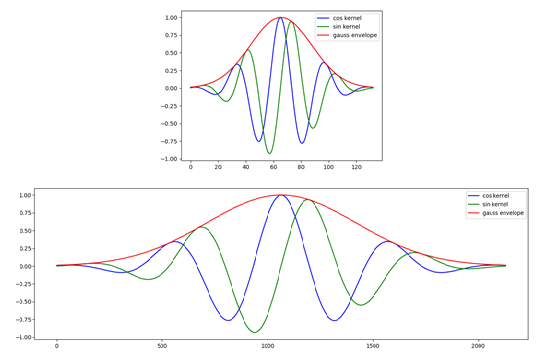
\includegraphics[width=\columnwidth]{figures/phasor_pulse_short_long.png}
    \caption{Top: Short phasor pulse, resulting in a high resolution reconstruction. Bottom: Long phasor pulse, resulting in a low resolution reconstruction.}
    \label{fig:long_short_pulse}
\end{figure}


\subsection{Spatial Decomposition}

The second tool that must be developed for our proposed method is a computation and memory efficient method to decompose 3D space. For this, we draw upon the well known data structure, the \textit{octree}, first proposed by \cite{octree}. This is a data structure that represents an axis-aligned 3D volume as a tree. The root node of the tree represents the entire volume. Each node of the tree starting with the root node has eight children. Each child represents one octant of the space contained by its parent. Therefore, each of the eight children represent $\frac{1}{8}$ the volume of its parent. As the tree descends in depth, the volume of a voxel at the $n$th level of the tree (with the root being $n=0$) represents a volume of $(\frac{1}{8})^n$ of the entire volume. A diagram of the tree structure, taken from \cite{Laurmaa2016} is shown in figure \ref{fig:octree}.

\begin{figure}
    \centering
    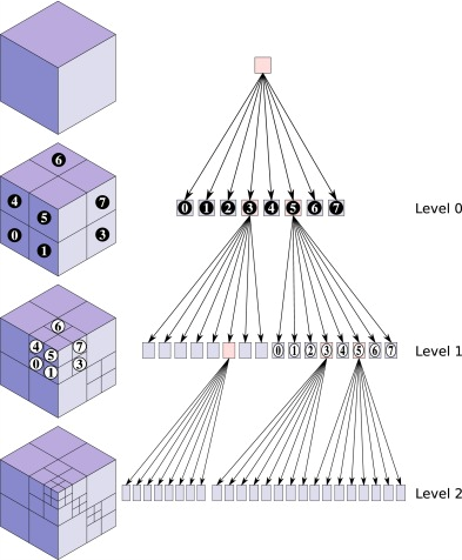
\includegraphics[width=\columnwidth]{figures/octree.png}
    \caption{Spatial decomposition by an octree data structure}
    \label{fig:octree}
\end{figure}

Implementation of our proposed method proceeds in the following manner. First, reconstruct the scene at a very coarse resolution. (In the limiting case, this would be reconstructing the scene as a single voxel). If there is sufficient signal present in this voxel, expand the octree by one level, dividing the current voxel into eight octants. For each of the eight octant voxels, reconstruct that voxel resolution and check if a sufficient signal is present. If a sufficient signal is not present, declare that voxel 'empty' and omit it from further processing. If the voxel has sufficient signal, repeat the process of subdividing and increasing the tree depth \textit{for that subtree} by one. Proceed until either all remaining voxels have been marked `empty,' or the tree depth produces leaf nodes whose voxels have dimension equal to the smallest possible reconstruction resolution of the source dataset. With this method, we identify large `empty' areas early and do not spend memory computational resources on reconstructing those areas at detailed resolution.

\section{Results}

The experimental portion of this work consisted of working with datasets collected by \cite{Liu2019}. Python code was developed to perform the virtual phasor field and backprojection as described in the Variable Resolution Reconstruction section above. An example of the construction at various resolutions can be seen in figure \ref{fig:multires}. This figure contains the 2D projection of the 3D reconstructions using the method described in the Background section. The convolution and backprojection algorithms were implemented using the \texttt{scipy} and \texttt{numpy} libraries, using vector operations everywhere possible, but running in a single thread. This implementation achieves performance results that exceed the reference Matlab/C++ implementation in \cite{Liu2019} when the C++ portion is run in single threaded mode. Significant opportunities for further optimization occur in performing the RSD convolution in frequency space, in performing the backprojection in parallel, and in general using GPU resources.

\begin{figure}
    \centering
        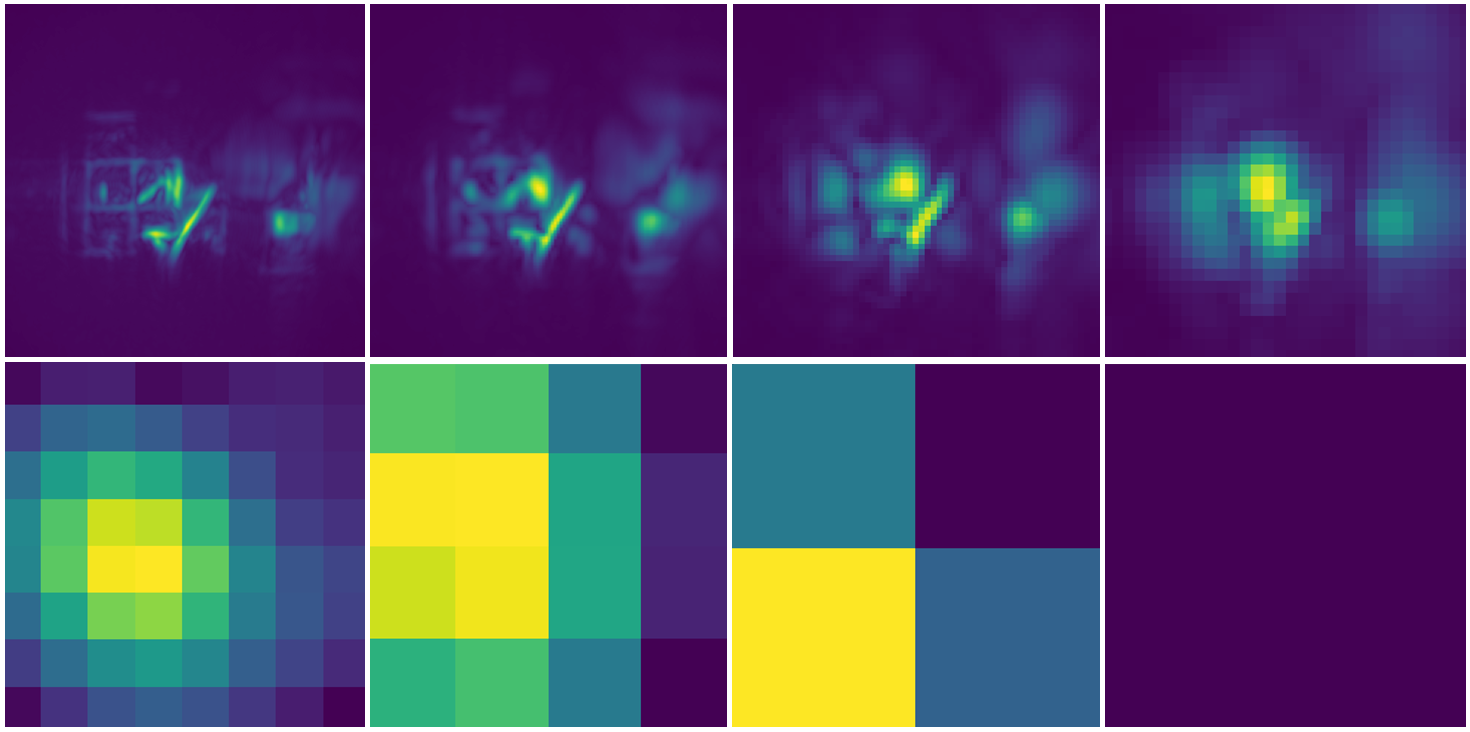
\includegraphics[width=\columnwidth]{figures/multires_2x4.png}
    \caption{Left: 2D Reconstruction of office scene at different resolutions. The top row from left to right is 1cm, 2cm, 4cm, and 8cm. The bottom row is 32cm, 64cm, 128cm, and 256cm. (16cm is not shown). The actual scene is 2.5m in each dimension, meaning the lowest resolution reconstruction (bottom right) is a single pixel (voxel).}
    \label{fig:multires}
\end{figure}

For the multi-resolution spatial decomposition portion of the investigation, we first assumed an ideal reconstruction at the finest possible resolution, where a single voxel in each Z-column is marked as having 'sufficient signal' and the remainder of voxels in that column are marked empty. This represents the ideal case, and a lower bound on the highest sparsity we could hope for in a reconstruction without noise or other artifacts. In our specific office scene dataset, this starting point was a 3D volume of size 2.5m x 2.5m x 2.3m, reconstructed at 1cm resolution, yielding a total of 14,375,000 voxels, of which 62,500 contain signal. A 3D view of the reconstructed scene prepared in this manner is shown in figure \ref{fig:3dscene}.

\begin{figure}
    \centering
        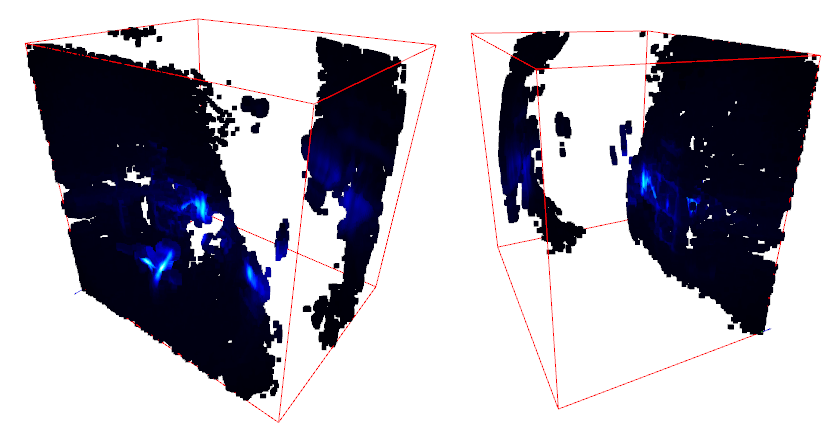
\includegraphics[width=0.8\columnwidth]{figures/3dscene.png}
    \caption{Left: Ideal reconstruction of office scene at 1cm resolution, front view. Right: Same scene, rear view.}
    \label{fig:3dscene}
\end{figure}

As can be seen in this figure, there are significant areas of the scene where even the highest intensity Z value for a given X,Y does not represent a meaningful object in the scene, for example the black pixels around the perimeter. These low-signal return voxels present an opportunity to exclude voxels from the scene that don't contribute to the semantic content of the image by means of a low-pass filter. Choosing a value empirically for the candidate scene results in a much more useful scene representation, shown in figure \ref{fig:threshold}.

\begin{figure}
    \centering
        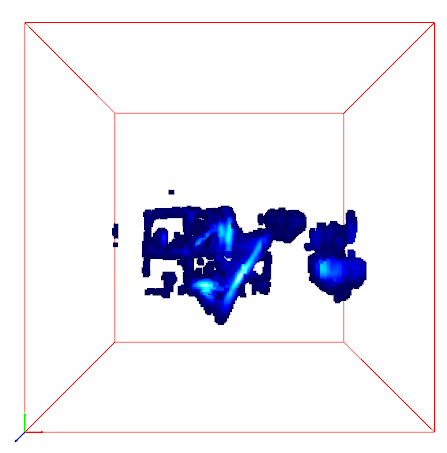
\includegraphics[width=0.6\columnwidth]{figures/threshold.png}
    \caption{Left: Ideal reconstruction of office scene at 1cm resolution, excluding low-signal return pixels}
    \label{fig:threshold}
\end{figure}

This ideal scene reconstruction was loaded into an octree data structure with visualization capabilities as provided by the Python \texttt{open3d} \cite{open3d} library. With this representation, the scene was regenerated using octrees with various maximal depths. Several of these depths are shown in figure \ref{fig:octree_depths}.  

\begin{figure}
    \centering
        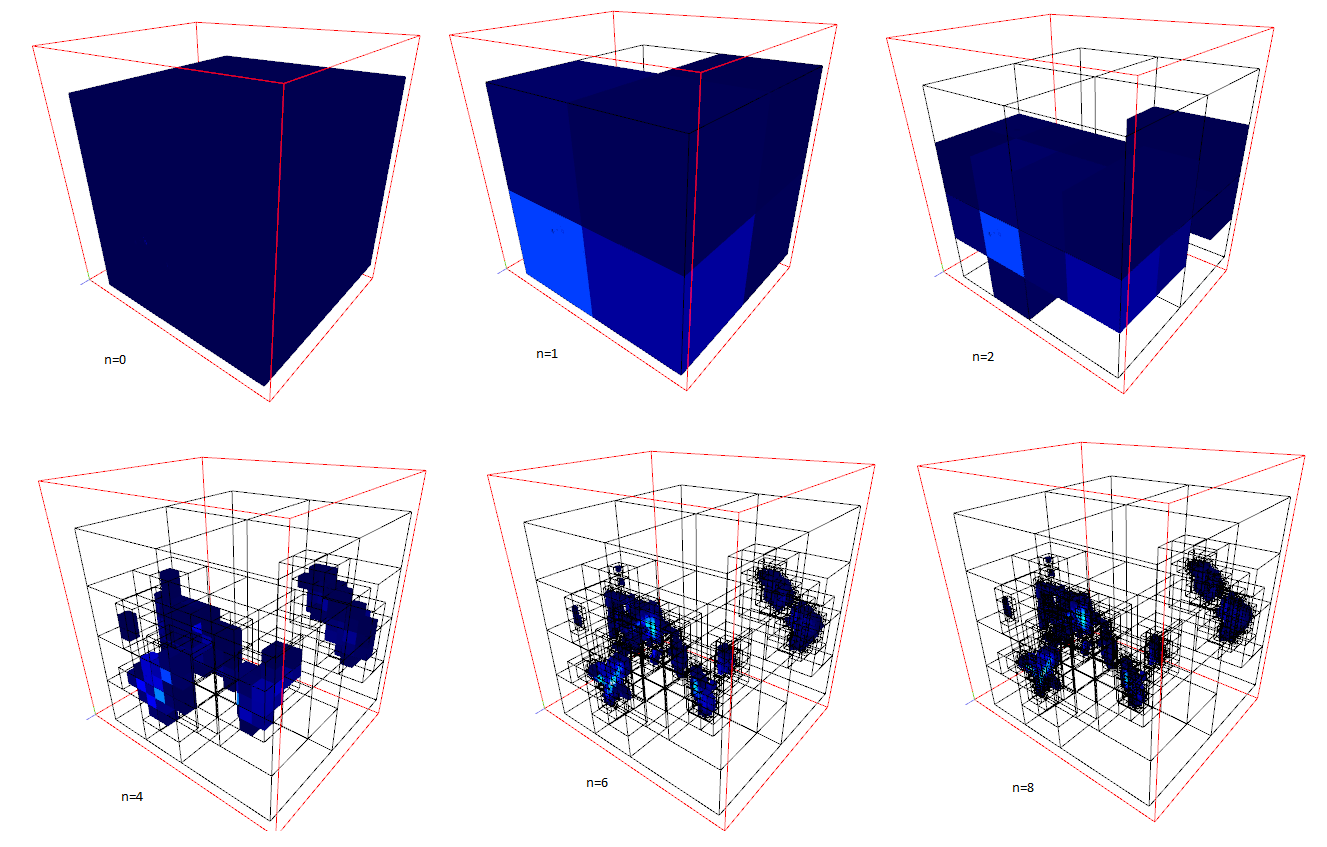
\includegraphics[width=\columnwidth]{figures/octree_depths.png}
    \caption{Left: Octree representation of the scene with various maximum depths}
    \label{fig:octree_depths}
\end{figure}

Our example scene has a dimension of 2.5m and a minimum reconstruction resolution of 1cm, meaning that when the octree reaches a depth of 8 (e.g. $2^8$ reductions in resolution), all original voxels that we want to represent will be located uniquely in leaf nodes of the tree. Statistics are calculated on the representation at the full spatial decomposition (depth = 8), and shown in table \ref{tab:stats} for both for with-pre-threshold and without-pre-threshold octree representations. As can be seen, with a reasonable pre-filter threshold value, it is possible that a complete reconstruction of the office scene using spatial decomposition would require only 55,625 voxel reconstructions instead of the full 14,375,000 reconstructions required if all 1cm voxels were reconstructed. This represents a substantial computational cost savings during the backprojection phase of the reconstruction.

\begin{table}[]
\centering
\begin{tabular}{@{}lcc@{}}
\toprule
                          & With Threshold & Without Threshold \\ \midrule
Maximum Depth             & 8              & 8                 \\
\# of Leaf Nodes      & 8,969          & 62,500            \\
\# of Internal Nodes  & 6,953          & 52,865            \\
\# of Empty Nodes     & 39,703         & 307,556           \\
\# of Reconstructions & 55,625         & 422,921           \\
\% Reconstructed          & 0.45\%         & 3.38\%            \\ \bottomrule
\end{tabular}
\caption{Octree statistics for office scene reconstruction}
\label{tab:stats}
\end{table}

\section{Limitations \& Future Work}

The work performed here and the proposed method is a proof-of-concept to demonstrate the potential gains of a complete implementation of the non-line of sight backrpojection reconstruction by means of spatial decomposition. There are multiple opportunities for improvement of method, and several unanswered practical questions before a complete implementation is feasible. 

The largest open question is determining the appropriate threshold at which the decision should be made to `declare empty' or `descend further.' In our simulation, this question was easily answered because the desired voxels to represent in the final tree were pre-computed during a full-resolution reconstruction. In practice, at each level of decomposition, the algorithm will need to determine whether the intensity value for that voxel represents a sufficiently large value that the interior should be subdivided and reconstructed. Finding this value may be a combination of theoretical and empirical work. The theoretical work may involve calculating the full expected intensity of the entire scene, and devising a bookkeeping method to determine how much has been accounted for already at other levels of the octree under construction. The threshold for descend/not-descend decision may even depend on z-depth of a voxel under consideration, as the signal fall-off with depth has recently been investigated by \cite{Nam2020}. This theoretical work could best be studied on simulated data, free of noise and higher order bounce artifacts. On the empirical side, it may be necessary to perform numerous experiments on existing data sets to understand and characterize the noise contributions to the scene.

Theoretical questions exist about the most efficient way to represent the virtual phasor field with multiple phasor field wavelengths. In the current work, each are stored separately in dense format. Choosing a sparse representation that is compact and easy to access will be important to  reducing memory footprint of the method. 

Implementation details also must be addressed. Modifications and additions will need to be made to the \texttt{open3d} library that supports the octree format. The current implementation chooses its root level dimensions based on the extents of the interior data supplied to it, rather than on an arbitrary work volume. Efficient use of GPU or other forms of parallel computing will still be necessary to fully utilize the processor capabilities of the host system. The current exploratory implementation is single threaded and CPU-only. Recursive descent through a tree structure should lend itself well to course-grained parallelism of multi-core CPUs, with individual voxel reconstruction being ideally suited for fine-grained parallelism of a GPU.

Currently, the scene reconstruction is done on a cartesian grid of voxels. It would be more appropriate to do the reconstruction in spherical coordinates with frustrum-shaped voxels that increase in size with increasing z-depth. The octree data structure would handle this sufficiently well, but the current implementation being used would require modifications.

An additional future possibility of the advantages of octree representation of a NLOS scene is to reconstruct different areas of the scene at different resolutions. This turns the `descend vs. not-descend' decision from a binary decision of `empty vs signal-present' to a multi-valued (or continuous) function of how important a particular area of a scene is deemed to be. Octree representation may be of significant utility if video (e.g. multi-frame) reconstruction with motion flow estimation is considered.

Ultimately, with the satisfactory resolution of the theoretical and practical questions raised above, the goal of this work should be to efficiently reconstruct scenes orders of magnitude larger than what is possible today. The encouraging results of this initial exploration suggest that this should indeed be possible.



%\begin{figure*}
%    \centering
%        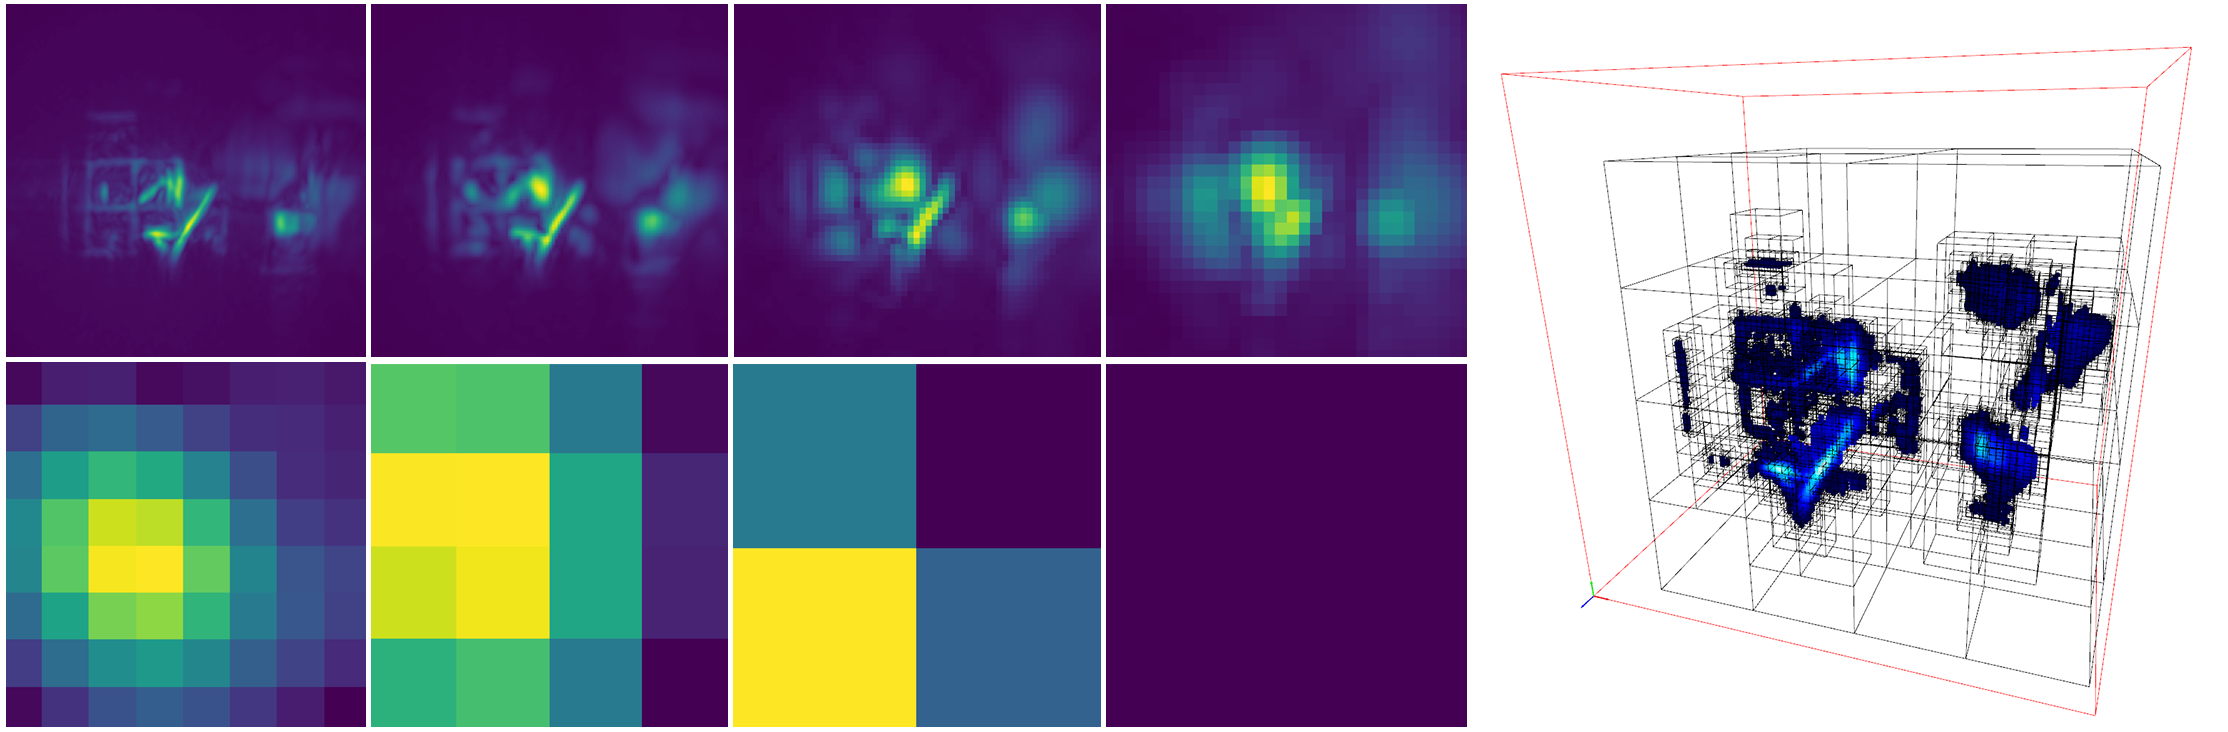
\includegraphics[width=2.0\columnwidth]{figures/teaser.png}
%    \caption{Left: 2D Reconstruction of office scene at different resolutions. Right: Octree spatial decomposition of same scene in 3D}
%    \label{fig:teaser}
%\end{figure*}


%\begin{figure*}
%    \centering
%        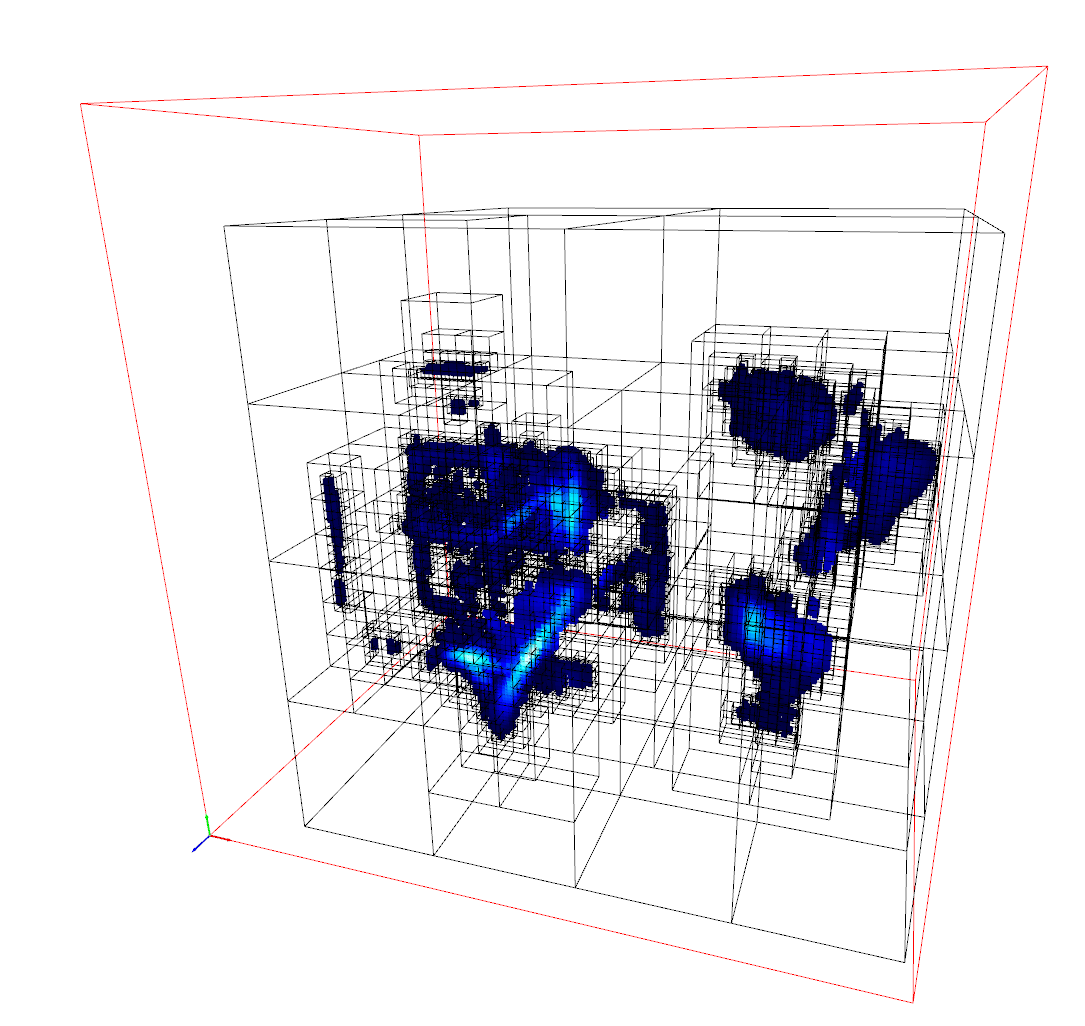
\includegraphics[width=1.0\columnwidth]{figures/officescene_octree.png}
%    \caption{Left: 2D Reconstruction of office scene at different resolutions. Right: Octree spatial decomposition of same scene in 3D}
%    \label{fig:teaser}
%\end{figure*}

%A plan to address other related work.

% An example of a floating figure using the graphicx package.
% Note that \label must occur AFTER (or within) \caption.
% For figures, \caption should occur after the \includegraphics.
% Note that IEEEtran v1.7 and later has special internal code that
% is designed to preserve the operation of \label within \caption
% even when the captionsoff option is in effect. However, because
% of issues like this, it may be the safest practice to put all your
% \label just after \caption rather than within \caption{}.
%
% Reminder: the "draftcls" or "draftclsnofoot", not "draft", class
% option should be used if it is desired that the figures are to be
% displayed while in draft mode.
%
%\begin{figure}[!t]
%\centering
%\includegraphics[width=2.5in]{myfigure}
% where an .eps filename suffix will be assumed under latex, 
% and a .pdf suffix will be assumed for pdflatex; or what has been declared
% via \DeclareGraphicsExtensions.
%\caption{Simulation results for the network.}
%\label{fig_sim}
%\end{figure}

% Note that the IEEE typically puts floats only at the top, even when this
% results in a large percentage of a column being occupied by floats.


% An example of a double column floating figure using two subfigures.
% (The subfig.sty package must be loaded for this to work.)
% The subfigure \label commands are set within each subfloat command,
% and the \label for the overall figure must come after \caption.
% \hfil is used as a separator to get equal spacing.
% Watch out that the combined width of all the subfigures on a 
% line do not exceed the text width or a line break will occur.
%
%\begin{figure*}[!t]
%\centering
%\subfloat[Case I]{\includegraphics[width=2.5in]{box}%
%\label{fig_first_case}}
%\hfil
%\subfloat[Case II]{\includegraphics[width=2.5in]{box}%
%\label{fig_second_case}}
%\caption{Simulation results for the network.}
%\label{fig_sim}
%\end{figure*}
%
% Note that often IEEE papers with subfigures do not employ subfigure
% captions (using the optional argument to \subfloat[]), but instead will
% reference/describe all of them (a), (b), etc., within the main caption.
% Be aware that for subfig.sty to generate the (a), (b), etc., subfigure
% labels, the optional argument to \subfloat must be present. If a
% subcaption is not desired, just leave its contents blank,
% e.g., \subfloat[].


% An example of a floating table. Note that, for IEEE style tables, the
% \caption command should come BEFORE the table and, given that table
% captions serve much like titles, are usually capitalized except for words
% such as a, an, and, as, at, but, by, for, in, nor, of, on, or, the, to
% and up, which are usually not capitalized unless they are the first or
% last word of the caption. Table text will default to \footnotesize as
% the IEEE normally uses this smaller font for tables.
% The \label must come after \caption as always.
%
%\begin{table}[!t]
%% increase table row spacing, adjust to taste
%\renewcommand{\arraystretch}{1.3}
% if using array.sty, it might be a good idea to tweak the value of
% \extrarowheight as needed to properly center the text within the cells
%\caption{An Example of a Table}
%\label{table_example}
%\centering
%% Some packages, such as MDW tools, offer better commands for making tables
%% than the plain LaTeX2e tabular which is used here.
%\begin{tabular}{|c||c|}
%\hline
%One & Two\\
%\hline
%Three & Four\\
%\hline
%\end{tabular}
%\end{table}


% Note that the IEEE does not put floats in the very first column
% - or typically anywhere on the first page for that matter. Also,
% in-text middle ("here") positioning is typically not used, but it
% is allowed and encouraged for Computer Society conferences (but
% not Computer Society journals). Most IEEE journals/conferences use
% top floats exclusively. 
% Note that, LaTeX2e, unlike IEEE journals/conferences, places
% footnotes above bottom floats. This can be corrected via the
% \fnbelowfloat command of the stfloats package.

% conference papers do not normally have an appendix


% use section* for acknowledgment
%\section*{Acknowledgment}
%The authors would like to thank...

% trigger a \newpage just before the given reference
% number - used to balance the columns on the last page
% adjust value as needed - may need to be readjusted if
% the document is modified later
%\IEEEtriggeratref{8}
% The "triggered" command can be changed if desired:
%\IEEEtriggercmd{\enlargethispage{-5in}}

% references section
\bibliographystyle{IEEEtran}
\bibliography{IEEEabrv,ref_final}

% that's all folks
\end{document}

